\documentclass[a4j, dvipdfm]{jarticle}
\usepackage[utf8]{inputenc}     %欧文でutf-8対応にする
\usepackage[hang,small,bf]{caption}
\usepackage[subrefformat=parens]{subcaption}

\usepackage{amsmath,amssymb}    %数式
\usepackage{bm}                 %太字ベクトル
\usepackage{graphicx}           %図の挿入
\usepackage{here}               %図の[H]を使えるようにする
\usepackage{ascmac}             %枠を使う
\usepackage{physics}            %コマンドの略称を用いる
\usepackage{comment}            %コメントの使用
\usepackage{enumerate}          %箇条書きを可能に
\usepackage{url}                %urlの利用
\usepackage{listings,jvlisting}
\usepackage[dvipdfmx]{hyperref}

% \usepackage{pxjahyper}

\pagestyle{empty}
\begin{document}
{\Large コンピュータ物理学}
\hskip1zw \hfill
\underline{ 3年 \hskip2zw \hskip2zw 学籍番号: 05502231\hskip3zw 氏名  松田愛理\hskip15ex }
\vspace*{2ex}


\begin{enumerate}[問題(1)]
  \large \item 使用コード\\
        \begin{flushleft}
          \href{https://github.com/eri61/computer_physics/tree/main/report1/code/report01_05502231Matsuda.ipynb}{jupyter notebook:}\\
          \href{https://github.com/eri61/computer_physics/blob/main/report1/code/func_solve_newton.py}{関連コード: func\_solve\_newton.py}\\
          \href{https://github.com/eri61/computer_physics/blob/main/report1/code/other_module.py}{関連コード: other\_module.py}\\
          ※コードはクリックで飛べます。
        \end{flushleft}
        \hspace{1cm}

        \large \item オイラー法の説明\\

        オイラー法とは、一階の微分方程式
        \begin{align}
          \frac{\mathrm{d}y(t)}{\mathrm{d}t} = f(t, y)
        \end{align}
        について、ある時刻$t_n$での変化量$f(t_n, y_n)$から任意の時刻での$y$の値を求める方法。既知の値$y(t_n)$から時刻$h$だけ進めた時の$y(t)$の値を$y_{t_n +h}$とする。この時、この$y_{t_n +h}$の展開は下記のようにあらわせる。
        \begin{align}
          y(t_n + h) & = y(t_n) + h \left(\frac{\mathrm{d}y(t)}{\mathrm{d}t}\right)_{t=t_n} + \mathcal{O}(h^2) \\
                     & \simeq y(t_n) + h \left(\frac{\mathrm{d}y(t)}{\mathrm{d}t}\right)_{t=t_n}
        \end{align}
        このことから、時刻$t_n$での値を用いると線形的に時刻$t_{n+1}$での値が近似できる。つまり初期値$t=t_{start}$、および$y(t)=y_0$を与えることにより任意の時刻での$y$の値$y(t)$が得られる。

        なお、Euler法により得られる誤差は$\mathcal{O}(h^2)$程度である。

        \begin{figure}[H]
          \centering
          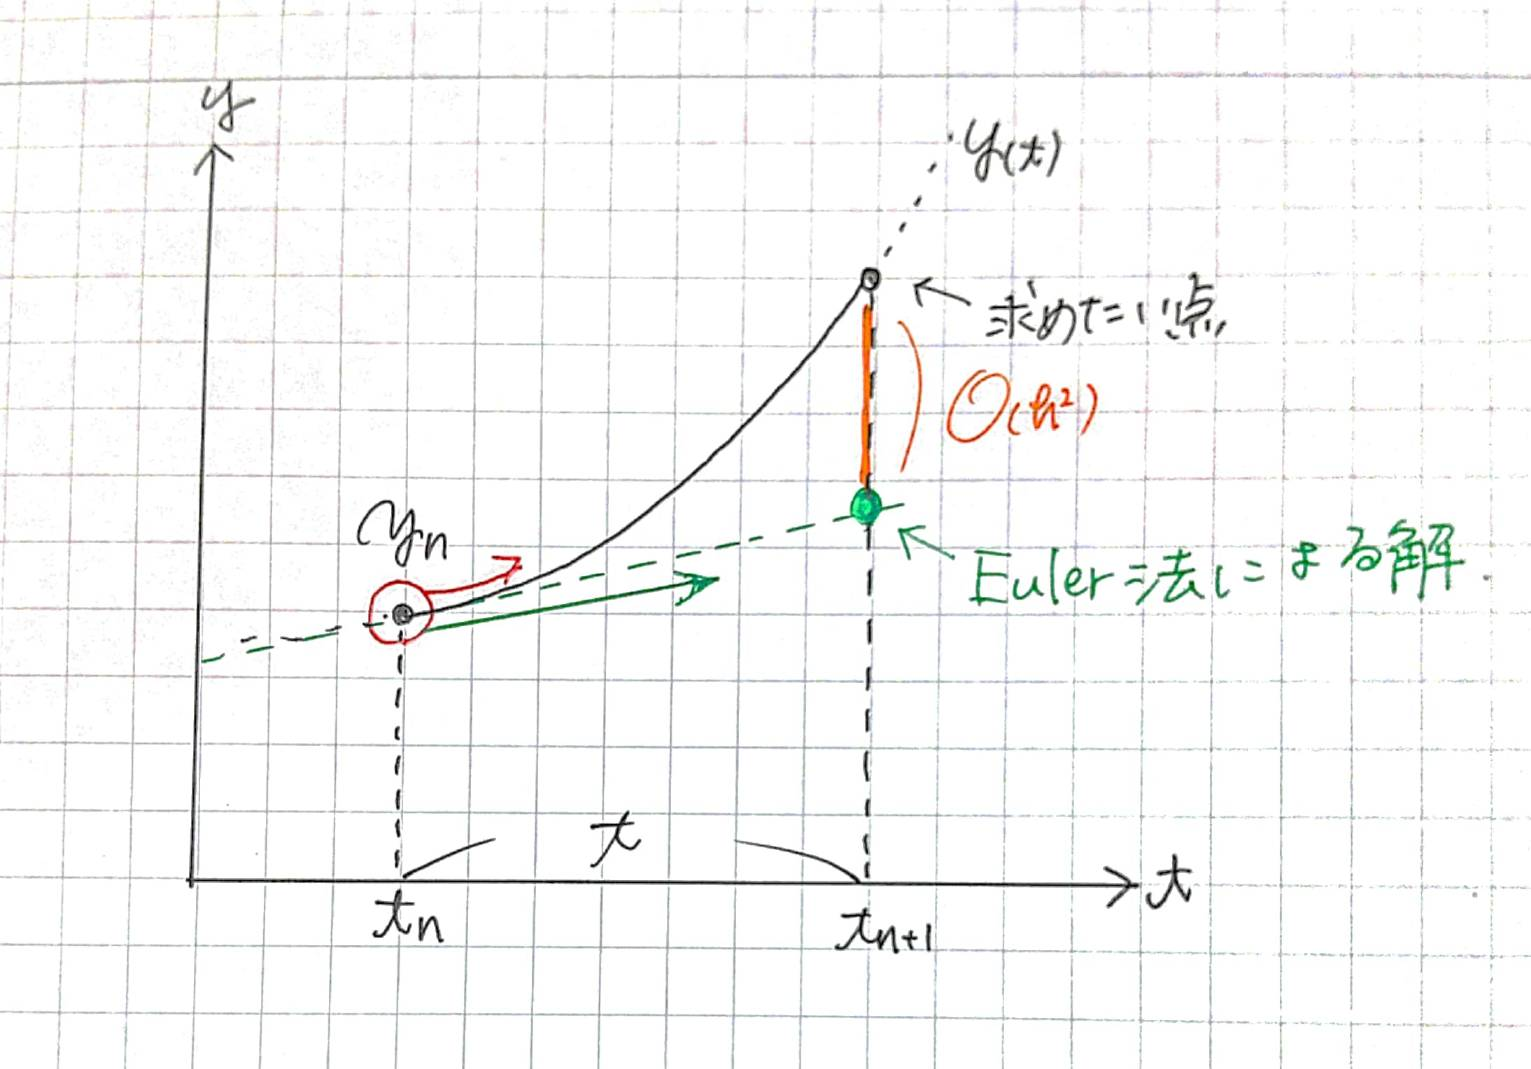
\includegraphics[height=8cm]{pic/5716.jpg}
          \caption{オイラー法}
          \label{}
        \end{figure}

        \large \item 抵抗係数と角度$\theta$の関係 \\
        (1)$L$と$\theta$の関係性を求める。質量$m$、抵抗係数$b$、初速度$v_0$の値をそれぞれ$m=0.1$、$b=0.1$、$v_0=100/3.6$としscipyのsolve\_inp関数を用いて抵抗のある運動方程式を解いた。結果のグラフは図\ref{L_theta}の通りとなった。
        \begin{alignat}{3}
          m\frac{\mathrm{d}v_x}{dt}       & = - bv_x    \hspace*{1cm}
                                          & m\frac{\mathrm{d}v_y}   {dt}    & = - bv_y - mg   \label{vx} \\
          \frac{\mathrm{d}x}{\mathrm{d}t} & = v_x,
                                          & \frac{\mathrm{d}y}{\mathrm{d}t} & = v_y \label{vy}
        \end{alignat}
        なお、垂直方向$y$、および水平方向$x$にの運動方程式には式(\ref{vx})(\ref{vy})を用いている。

        \begin{figure}[H]
          \centering
          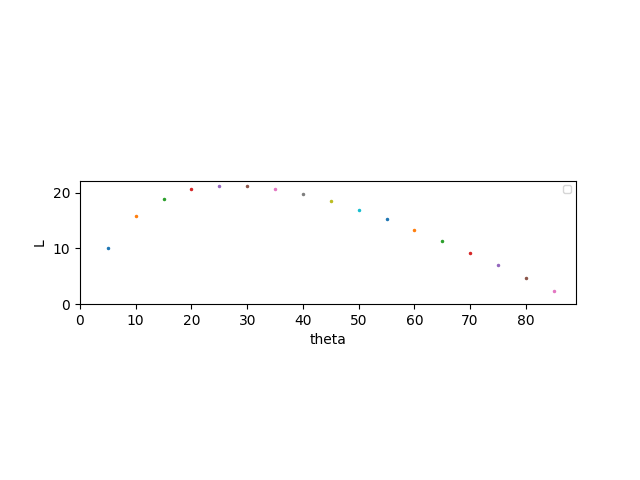
\includegraphics[height=5cm]{pic/related_theta_L.png}
          \caption{到達距離$L$と$\theta$の関係}
          \label{L_theta}
        \end{figure}

        (2)最大到達距離$L_{max}$とその時の角度$\theta$ \\
        次に、最大到達距離$L_{max}$を誇る放射角度$\theta_{max}$と抵抗係数$b/m$の関係を計算した。図\ref{change_bm}は抵抗係数$b/m$を変更したときの到達距離$L$と放射角度$\theta$を表している。
        \begin{figure}[H]
          \centering
          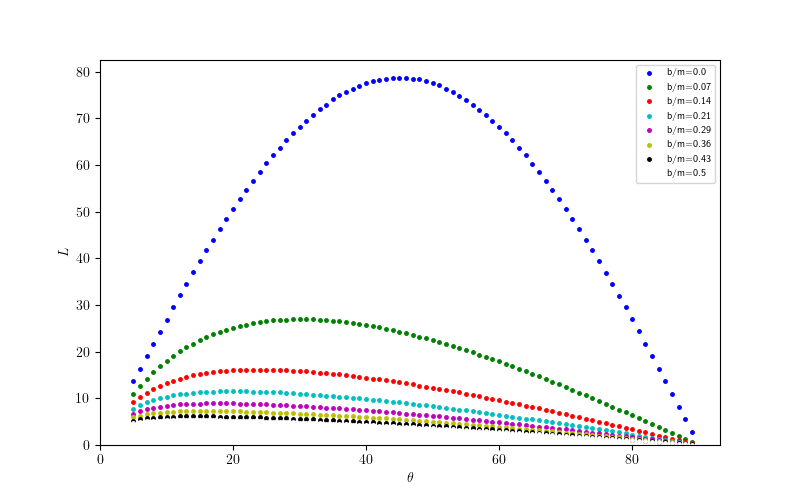
\includegraphics[width=12cm]{pic/change_bm.png}
          \caption{抵抗係数$b/m$を変えた時の到達距離$L$と角度$\theta$の関係}
          \label{change_bm}
        \end{figure}

        図\ref{change_bm}から、抵抗が大きくなるに従って最大到達距離が小さくなり、同時にの到達距離$L_{max}$の時の放射角も小さくなっている(だんだん凸部が左に寄ったグラフになっている)ことが分かる。

        最後に、放射角度$\theta_{max}$と抵抗係数$b/m$の値を抽出し、図示を行った。結果は図\ref{theta_max}の通りになった。
        \begin{figure}[H]
          \centering
          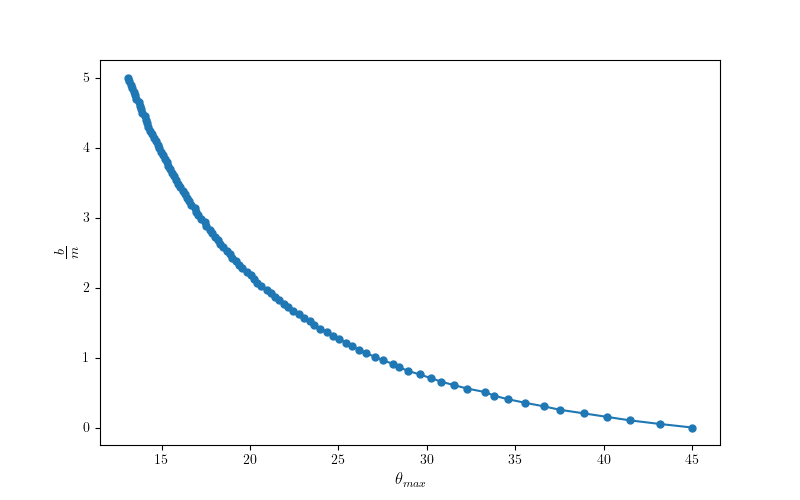
\includegraphics[width=12cm]{pic/related_theta_bm.png}
          \caption{}
          \label{theta_max}
        \end{figure}
        図\ref{theta_max}の結果は抵抗係数$b/m=0$の時に$\theta_{max}=45$°、抵抗係数が無限大で十分大きくなると$\theta_{max}=0$に近づき、直感的な解釈と合致する。

        \vspace{0.5cm}
        なお、この計算では抵抗係数は$0.0\sim 5.0$の内$50$個の点を取り、対応するそれぞれの方程式に対し、放射角度$0\sim 90$°を$400$個に分割するようにして計算を行った。計算速度の都合上実際には$400$分割を行うのではなく、一度$20$分割を行い最適な$\theta_{max}$を導出してから、その周辺$\pm 1/20$について再度$40$分割を行っている。
        最終的な最大到達距離には、図\ref{L_theta}のようなグラフの到達距離$L$が最大となる4つの点を抽出し、curve\_fit関数により2次関数のフィッティングを行っている。


\end{enumerate}
\end{document}